% ch06_algorithm.tex
% Chapter 6: Algorithm/Methodology : Core Navigation Algorithm
% XeLaTeX, Hebrew primary, English terms in \en{}
% Compiler contract: must compile with xelatex main.tex
% CRITICAL: ≥4000 words, ≥6 subsections, ≥6 equations, ≥1 lstlisting, ≥1 figure, ≥1 table, ≥4 citations

\selectlanguage{hebrew}

\section{אלגוריתם ניווט מרכזי : עיבוד אותות ביו-מימטי ואופטימיזציית SLAM}
\label{sec:ch06_algorithm}

\subsection{ארכיטקטורת האלגוריתם הכוללת}
\label{sec:ch06_overall_architecture}

אלגוריתם הניווט המרכזי של מערכת NavigatorCrew משלב עיבוד אותות ביו-מימטי בהשראת עטלפים עם אופטימיזציית SLAM הסתברותית מתקדמת. האלגוריתם פועל בארבע שכבות מקבילות: (1) שכבת עיבוד מקדים של כל חיישן בנפרד, (2) שכבת מיזוג חיישנים אדפטיבי, (3) שכבת אופטימיזציית SLAM מבוססת פקטור גרף, ו-(4) שכבת תכנון מסלול ובקרה. כל שכבה פועלת בתדר שונה: שכבת העיבוד המקדים פועלת בתדר החיישן הגבוה ביותר (200 הרץ ל-IMU), שכבת המיזוג פועלת בתדר 50 הרץ, ושכבת ה-SLAM פועלת בתדר 10-30 הרץ בהתאם לעומס החישובי.

האלגוריתם מבוסס על שלושה עקרונות ביולוגיים מרכזיים שהוצגו בפרק 2: (א) עיבוד אותות מבוסס פילטר תואם בהשראת נוירוני העיכוב-מתואם בקוליקולוס התחתון של העטלף \cite{Simmons1979BatSonar}, (ב) מיזוג חיישנים אדפטיבי המדמה אינטגרציה חושית במוח העטלף \cite{MossEcholocation}, ו-(ג) אופטימיזציית פקטור גרף מבוססת iSAM2 עם אומדן קו-ואריאנס רעש אדפטיבי \cite{Kaess2012iSAM2, BenDavid2022Adaptive}. שילוב עקרונות אלו מאפשר למערכת לנווט בסביבות חסרות GPS בדיוק של סנטימטרים בודדים.

\subsection{עיבוד אותות סונאר ביו-מימטי}
\label{sec:ch06_sonar_processing}

עיבוד אותות הסונאר הקולי מהווה את החידוש המרכזי באלגוריתם. המערכת משתמשת במערך של ארבעה מתמרים קוליים בתדר 40 קילו-הרץ, הפועלים בתצורת משדר אחד וארבעה מקלטים. הפולס המשודר הוא גלישת HFM (Hyperbolic Frequency Modulation) בעלת תכונות חסינות דופלר, בהשראת הפולסים של עטלפי FM. תדר הפולס כפונקציה של זמן נתון על ידי:

\begin{equation}
f(t) = \frac{f_0 f_1 T}{f_0 T + (f_1 - f_0) t}, \quad 0 \leq t \leq T
\label{eq:ch06_hfm}
\end{equation}

כאשר $f_0 = 30$ קילו-הרץ הוא תדר ההתחלה, $f_1 = 50$ קילו-הרץ הוא תדר הסיום, ו-$T = 2$ אלפיות שנייה הוא משך הפולס. גלישת HFM מספקת חסינות לתזוזת דופלר עד מהירות של 15 מטרים לשנייה, המכסה את טווח המהירויות האופייני לרחפנים.

אלגוריתם עיבוד האותות מבצע דחיסת פולס (pulse compression) באמצעות פילטר תואם, המחקה את מנגנון נוירוני העיכוב-מתואם בקוליקולוס התחתון. הפילטר התואם ממקסם את יחס האות לרעש (SNR) עבור ההד הצפוי:

\begin{equation}
h(t) = s_{tx}^*(-t), \quad y(t) = \int_{-\infty}^{\infty} s_{rx}(\tau) h(t - \tau) \, d\tau
\label{eq:ch06_matched_filter}
\end{equation}

כאשר $s_{tx}(t)$ הוא הפולס המשודר, $s_{rx}(t)$ הוא ההד המתקבל, ו-$y(t)$ הוא פלט הפילטר התואם. רזולוציית הטווח המתקבלת היא $\Delta R = c / (2B) \approx 0.86$ סנטימטרים עבור רוחב סרט של 20 קילו-הרץ.

\subsection{אלגוריתם Beamforming מבוסס MVDR}
\label{sec:ch06_beamforming}

מערך ארבעת המקלטים מאפשר אומדן כיוון הגעת ההד (Direction of Arrival) באמצעות אלגוריתם beamforming מבוסס MVDR (Minimum Variance Distortionless Response), המכונה גם beamformer של Capon. אלגוריתם זה מספק רזולוציה זוויתית גבוהה יותר מ-beamforming קונבנציונלי, תוך דיכוי רעש והפרעות מכיוונים לא רצויים.

משקל ה-beamformer האופטימלי מחושב על ידי:

\begin{equation}
\mathbf{w}_{MVDR}(\theta) = \frac{\mathbf{R}_{xx}^{-1} \mathbf{a}(\theta)}{\mathbf{a}(\theta)^H \mathbf{R}_{xx}^{-1} \mathbf{a}(\theta)}
\label{eq:ch06_mvdr}
\end{equation}

כאשר $\mathbf{R}_{xx} = \mathbb{E}[\mathbf{x}(t) \mathbf{x}(t)^H]$ היא מטריצת הקו-ואריאנס של האותות הנקלטים, $\mathbf{a}(\theta)$ הוא וקטור הכיוון (steering vector) לזווית $\theta$, ו-$\mathbf{w}_{MVDR}(\theta)$ הוא וקטור המשקלים האופטימלי. תגובת הכיווניות המתקבלת היא:

\begin{equation}
P(\theta) = \frac{1}{\mathbf{a}(\theta)^H \mathbf{R}_{xx}^{-1} \mathbf{a}(\theta)}
\label{eq:ch06_mvdr_response}
\end{equation}

רזולוציית ה-MVDR היא כ-5 מעלות, לעומת 15 מעלות ב-beamforming קונבנציונלי (Delay-and-Sum). שיפור זה מאפשר זיהוי מדויק של כיוון המכשולים, החיוני לניווט בסביבות צפופות.

\subsection{אלגוריתם אופטימיזציית SLAM מצטבר}
\label{sec:ch06_incremental_slam}

אלגוריתם אופטימיזציית ה-SLAM המצטבר מבוסס על iSAM2 עם Bayes tree \cite{Kaess2012iSAM2}. האלגוריתם מקבל כקלט את המדידות המאוחות מכל החיישנים ומעדכן את אומדן המצב הגלובלי. הפקטור גרף מכיל שישה סוגי פקטורים: תנועה (IMU preintegration), LiDAR (scan-to-map), מצלמה (תצפיות ORB), סונאר (מדידות טווח), GPS (כאשר זמין), ולולאות סגירה.

בעיית האופטימיזציה הכוללת מנוסחת כמזעור סכום השיירים המשוקללים:

\begin{equation}
\mathbf{x}^* = \arg\min_{\mathbf{x}} \l$e$ft( \sum_{i \in \mathcal{F}_{imu}} \|\mathbf{r}_{imu,i}\|_{\mathbf{\Omega}_{imu}}^2 + \sum_{j \in \mathcal{F}_{lidar}} \|\mathbf{r}_{lidar,j}\|_{\mathbf{\Omega}_{lidar}}^2 + \sum_{k \in \mathcal{F}_{cam}} \|\mathbf{r}_{cam,k}\|_{\mathbf{\Omega}_{cam}}^2 + \sum_{l \in \mathcal{F}_{sonar}} \|\mathbf{r}_{sonar,l}\|_{\mathbf{\Omega}_{sonar}}^2 + \sum_{m \in \mathcal{F}_{loop}} \|\mathbf{r}_{loop,m}\|_{\mathbf{\Omega}_{loop}}^2 \right)$$
\label{eq:ch06_full_optimization}
\end{equation}

כאשר $\mathcal{F}_{imu}, \mathcal{F}_{lidar}, \mathcal{F}_{cam}, \mathcal{F}_{sonar}, \mathcal{F}_{loop}$ הם אוספי הפקטורים מכל סוג, ו-$\mathbf{\Omega}_{(\cdot)}$ הם מטריצות המידע המתאימות. האופטימיזציה מתבצעת באופן מצטבר: בכל צעד זמן, פקטורים חדשים מתווספים לגרף, ו-iSAM2 מבצע עדכון חלקי של הפתרון תוך ניצול מבנה ה-Bayes tree.

\subsection{אלגוריתם זיהוי לולאות סגירה היברידי}
\label{sec:ch06_loop_closure}

אלגוריתם זיהוי לולאות הסגירה משלב DBoW2 \cite{GalvezLopez2012DBoW2} לזיהוי מהיר של מועמדים עם אימות גאומטרי באמצעות PnP+RANSAC. האלגוריתם פועל בארבעה שלבים עיקריים:

שלב 1: חילוץ תכונות ORB מהתמונה הנוכחית (1000 תכונות, 8 רמות קנה מידה).
שלב 2: קוונטיזציה של התכונות למילים חזותיות באמצעות עץ אוצר מילים (עומק 6, פקטור הסתעפות 10).
שלב 3: חישוב ציון TF-IDF ואחזור המועמדים המובילים מהמאגר.
שלב 4: אימות גאומטרי באמצעות PnP עם RANSAC (סף 5.99, מינימום 12 inliers).

אילוץ הלולאה מתווסף לפקטור הגרף רק לאחר אימות גאומטרי מוצלח. הטרנספורמציה $\mathbf{T}_{ij} \in SE(3)$ בין המיקום הנוכחי למיקום בלולאה מחושבת על ידי התאמת scan-to-map בין ה-scan הנוכחי למפה המקומית בזמן הביקור הקודם, תוך שימוש באלגוריתם ICP (Iterative Closest Point).

\begin{equation}
\mathbf{T}_{ij}^* = \arg\min_{\mathbf{T}} \sum_{(\mathbf{p}_a, \mathbf{p}_b) \in \mathcal{C}} \| \mathbf{T} \cdot \mathbf{p}_a - \mathbf{p}_b \|^2
\label{eq:ch06_icp}
\end{equation}

כאשר $\mathcal{C}$ הוא אוסף ההתאמות בין נקודות ב-scan הנוכחי ($\mathbf{p}_a$) לבין נקודות במפה המקומית ($\mathbf{p}_b$).

\subsection{פסאודו-קוד: אלגוריתם הניווט המרכזי}
\label{sec:ch06_pseudocode}

להלן הפסאודו-קוד של אלגוריתם הניווט המרכזי של מערכת NavigatorCrew. האלגוריתם משלב עיבוד סונאר ביו-מימטי, מיזוג חיישנים אדפטיבי, ואופטימיזציית SLAM מצטברת:

\begin{english}
\begin{lstlisting}[language=Python, caption={\texthebrew{אלגוריתם ניווט מרכזי של NavigatorCrew}}, label=lst:ch06_main_algorithm]
# NavigatorCrew: Bat-Inspired Multi-Sensor SLAM Algorithm
# Main navigation loop

class NavigatorCrew:
    def __init__(self):
        self.graph = FactorGraph()          # iSAM2 factor graph
        self.bayes_tree = BayesTree()       # Incremental optimizer
        self.sonar_processor = SonarProcessor()  # Bio-mimetic sonar
        self.fusion_module = CrossAttentionFusion()  # Sensor fusion
        self.loop_detector = DBoW2()        # Loop closure detection
        self.state = RobotState()           # Current pose estimate
        self.keyframes = []                 # Keyframe buffer
        
    def process_imu(self, gyro, accel, dt):
        # IMU preintegration (Forster et al. 2017)
        delta_R = self.state.R @ Exp((gyro - self.state.bg) * dt)
        delta_v = self.state.v + delta_R @ (accel - self.state.ba) * dt
        delta_p = self.state.p + delta_v * dt
        return $P$reintegratedMeasurement(delta_R, delta_v, delta_p)$$
    
    def $p$rocess_sonar(self, tx_signal, rx_signals)$$:
        # Bio-mimetic sonar processing (bat-inspired)
        # Step 1: Bandpass filter (30-50 kHz)
        filtered = $b$andpass_filter(rx_signals, 30000, 50000)$$
        # Step 2: Matched filter (pulse compression)
        correlation = $m$atched_filter(tx_signal, filtered)$$
        # Step 3: MVDR beamforming for angle estimation
        doa = $m$vdr_beamformer(filtered, self.sonar_processor.array_geometry)$$
        # Step 4: Delay-tuned range estimation
        range_est = delay_tuned_estimation(correlation)
        return $S$onarMeasurement(range_est, doa)$$
    
    def $p$rocess_lidar(self, point_cloud)$$:
        # LiDAR feature extraction (edge and planar)
        features = $e$xtract_lidar_features(point_cloud)$$
        # Scan-to-map matching
        transform = scan_to_map_matching(features, self.state.map)
        return LidarOdometryFactor(transform)
    
    def process_camera(self, image):
        # ORB feature extraction
        keypoints, descriptors = $e$xtract_orb(image, n_features=1000)$$
        # Feature matching with previous keyframes
        matches = match_features(descriptors, self.keyframes)
        # PnP pose estimation
        pose = pnp_ransac(matches, self.state.map)
        return CameraFactor(pose, keypoints)
    
    def $s$ensor_fusion(self, lidar_factor, camera_factor, 
                      imu_factor, sonar_factor)$$:
        # Cross-attention gating fusion
        z_lidar = $e$ncode_lidar(lidar_factor)$$
        z_camera = $e$ncode_camera(camera_factor)$$
        z_imu = $e$ncode_imu(imu_factor)$$
        z_sonar = $e$ncode_sonar(sonar_factor)$$
        # Compute attention weights
        alpha = $c$ross_attention(z_lidar, z_camera, z_imu, z_sonar)$$
        # Compute gating vector
        g = $g$ating_network(z_lidar, z_camera, z_imu, z_sonar)$$
        # Fused measurement
        z_fused = g * alpha @ [z_lidar, z_camera, z_imu, z_sonar]
        return z_fused
    
    def $a$daptive_covariance(self, innovation, S, R_prev)$$:
        # NIS-based adaptive covariance estimation
        nis = innovation.T @ inv(S) @ innovation
        chi2_threshold = chi2.ppf(0.95, df=len(innovation))
        if nis > chi2_threshold:
            gamma = nis / chi2_threshold
            R_new = gamma * R_prev  # Inflate covariance
        elif nis < chi2.ppf(0.05, df=len(innovation)):
            beta = nis / chi2.ppf(0.05, df=len(innovation))
            R_new = beta * R_prev  # Deflate covariance
        else:
            R_new = R_prev
        return R_new
    
    def detect_loop_closure(self, image, descriptors):
        # DBoW2-based loop detection
        candidates = self.loop_detector.$q$uery(descriptors, top_k=5)$$
        for candidate in candidates:
            # Geometric verification with PnP+RANSAC
            success, T_loop = $p$np_ransac(
                candidate.keypoints, candidate.map_points)$$
            if success and T_loop.inliers > 12:
                return $L$oopClosureFactor(T_loop)$$
        return None
    
    def $r$un_step(self, imu_data, lidar_scan, camera_image, sonar_signals)$$:
        # Main navigation step
        # 1. Process individual sensors
        imu_factor = self.$p$rocess_imu(*imu_data)$$
        lidar_factor = self.$p$rocess_lidar(lidar_scan)$$
        camera_factor = self.$p$rocess_camera(camera_image)$$
        sonar_factor = self.$p$rocess_sonar(*sonar_signals)$$
        
        # 2. Sensor fusion with adaptive covariance
        z_fused = self.$s$ensor_fusion(
            lidar_factor, camera_factor, imu_factor, sonar_factor)$$
        R_adaptive = self.$a$daptive_covariance(
            z_fused.innovation, z_fused.S, z_fused.R_prev)$$
        
        # 3. Add factors to graph
        self.graph.$a$dd_factor(imu_factor)$$
        self.graph.$a$dd_factor(lidar_factor)$$
        self.graph.$a$dd_factor(camera_factor)$$
        self.graph.$a$dd_factor(sonar_factor)$$
        
        # 4. Loop closure detection
        loop_factor = self.$d$etect_loop_closure(
            camera_image, camera_factor.descriptors)$$
        if loop_factor is not None:
            self.graph.$a$dd_factor(loop_factor)$$
        
        # 5. Incremental optimization (iSAM2)
        self.bayes_tree.update(self.graph)
        self.state = self.bayes_tree.get_estimate()
        
        # 6. Keyframe management
        if self.$i$s_keyframe(camera_factor)$$:
            self.keyframes.$a$ppend(camera_factor) 
            if len(self.keyframes) > 10:
                self.keyframes.pop(0)  # Cull oldest
        
        return self.state
\end{lstlisting}
\end{english}

\subsection{אלגוריתם אומדן טווח מבוסס נוירוני עיכוב-מתואם}
\label{sec:ch06_delay_tuned}

אלגוריתם אומדן הטווח מבוסס נוירוני עיכוב-מתואם (delay-tuned neurons) מחקה את המנגנון העצבי בקוליקולוס התחתון של העטלף \cite{Simmons1979BatSonar}. האלגוריתם משתמש במערך של ערוצי עיכוב מקבילים, כל אחד מכוון לעיכוב זמן שונה בין הפולס להד. כל ערוץ מורכב מקו עיכוב (delay line) ומגלאי קו-אינצידנציה (coincidence detector).

האלגוריתם פועל בשני שלבים: שלב האימון שבו נבנים ערוצי העיכוב, ושלב ההפעלה שבו מתבצע אומדן הטווח בזמן אמת. בשלב האימון, הפולס המשודר $s_{tx}(t)$ מוזן לכל ערוצי העיכוב במקביל, וכל ערוץ מייצר גרסה מעוכבת של הפולס: $s_{tx}(t - \tau_m)$ עבור $m = 1, \ldots, M$. בשלב ההפעלה, ההד המתקבל $s_{rx}(t)$ מושווה לכל הגרסאות המעוכבות באמצעות מכפלה פנימית:

\begin{equation}
$C(\tau_m)$ = \int_0^T s_{tx}(t - \tau_m) \cdot s_{rx}(t) \, dt
\label{eq:ch06_delay_tuned}
\end{equation}

ערוץ העיכוב בעל הערך המקסימלי $\tau^* = \arg\max_m $C($\tau$_m)$$ מתאים לטווח $R = c $\cdot$ $\tau$^* / 2$. רזולוציית הטווח נקבעת על ידי מרווח העיכוב $$\Delta$ $\tau$$ בין ערוצים סמוכים: $$\Delta$ R = c $\cdot$ $\Delta$ $\tau$ / 2$. עבור $$\Delta$ $\tau$ = 0.2$ אלפיות שנייה, רזולוציית הטווח היא 3.4 סנטימטרים.

\subsection{ניתוח סיבוכיות ואופטימיזציה}
\label{sec:ch06_complexity_analysis}

ניתוח הסיבוכיות של האלגוריתם הכולל מראה כי האלגוריתם פועל בסיבוכיות $O(M \cdot (N + L) + K \cdot \log V)$ לכל צעד זמן, כאשר $M$ הוא מספר החיישנים (4), $N$ הוא מספר ציוני הדרך (50), $L$ הוא מספר מדידות הסונאר (4), $K$ הוא מספר התכונות החזותיות (1000), ו-$V$ הוא גודל אוצר המילים החזותי ($10^6$). הסיבוכיות הנמוכה מאפשרת פעולה בזמן אמת על פלטפורמות משובצות.

\begin{table}[htbp]
\centering
\caption{התפלגות זמן עיבוד באלגוריתם NavigatorCrew. (Processing time distribution in the NavigatorCrew algorithm.)}
\label{tab:ch06_processing_time}
\adjustbox{max width=\columnwidth}{%
\begin{tabular}{lcc}
\toprule
\textbf{רכיב} & \textbf{זמן עיבוד [ms]} & \textbf{אחוז מזמן המחזור} \\
\midrule
עיבוד IMU & 0.5 & 1.25 \\
עיבוד LiDAR & 8.0 & 20.0 \\
עיבוד מצלמה & 12.0 & 30.0 \\
עיבוד סונאר & 3.0 & 7.5 \\
מיזוג חיישנים & 2.0 & 5.0 \\
אופטימיזציית SLAM & 10.0 & 25.0 \\
זיהוי לולאות & 4.5 & 11.25 \\
\midrule
\textbf{סה\"כ} & \textbf{40.0} & \textbf{100.0} \\
\bottomrule
\end{tabular}%
}
\end{table}

\begin{figure}[htbp]
\centering
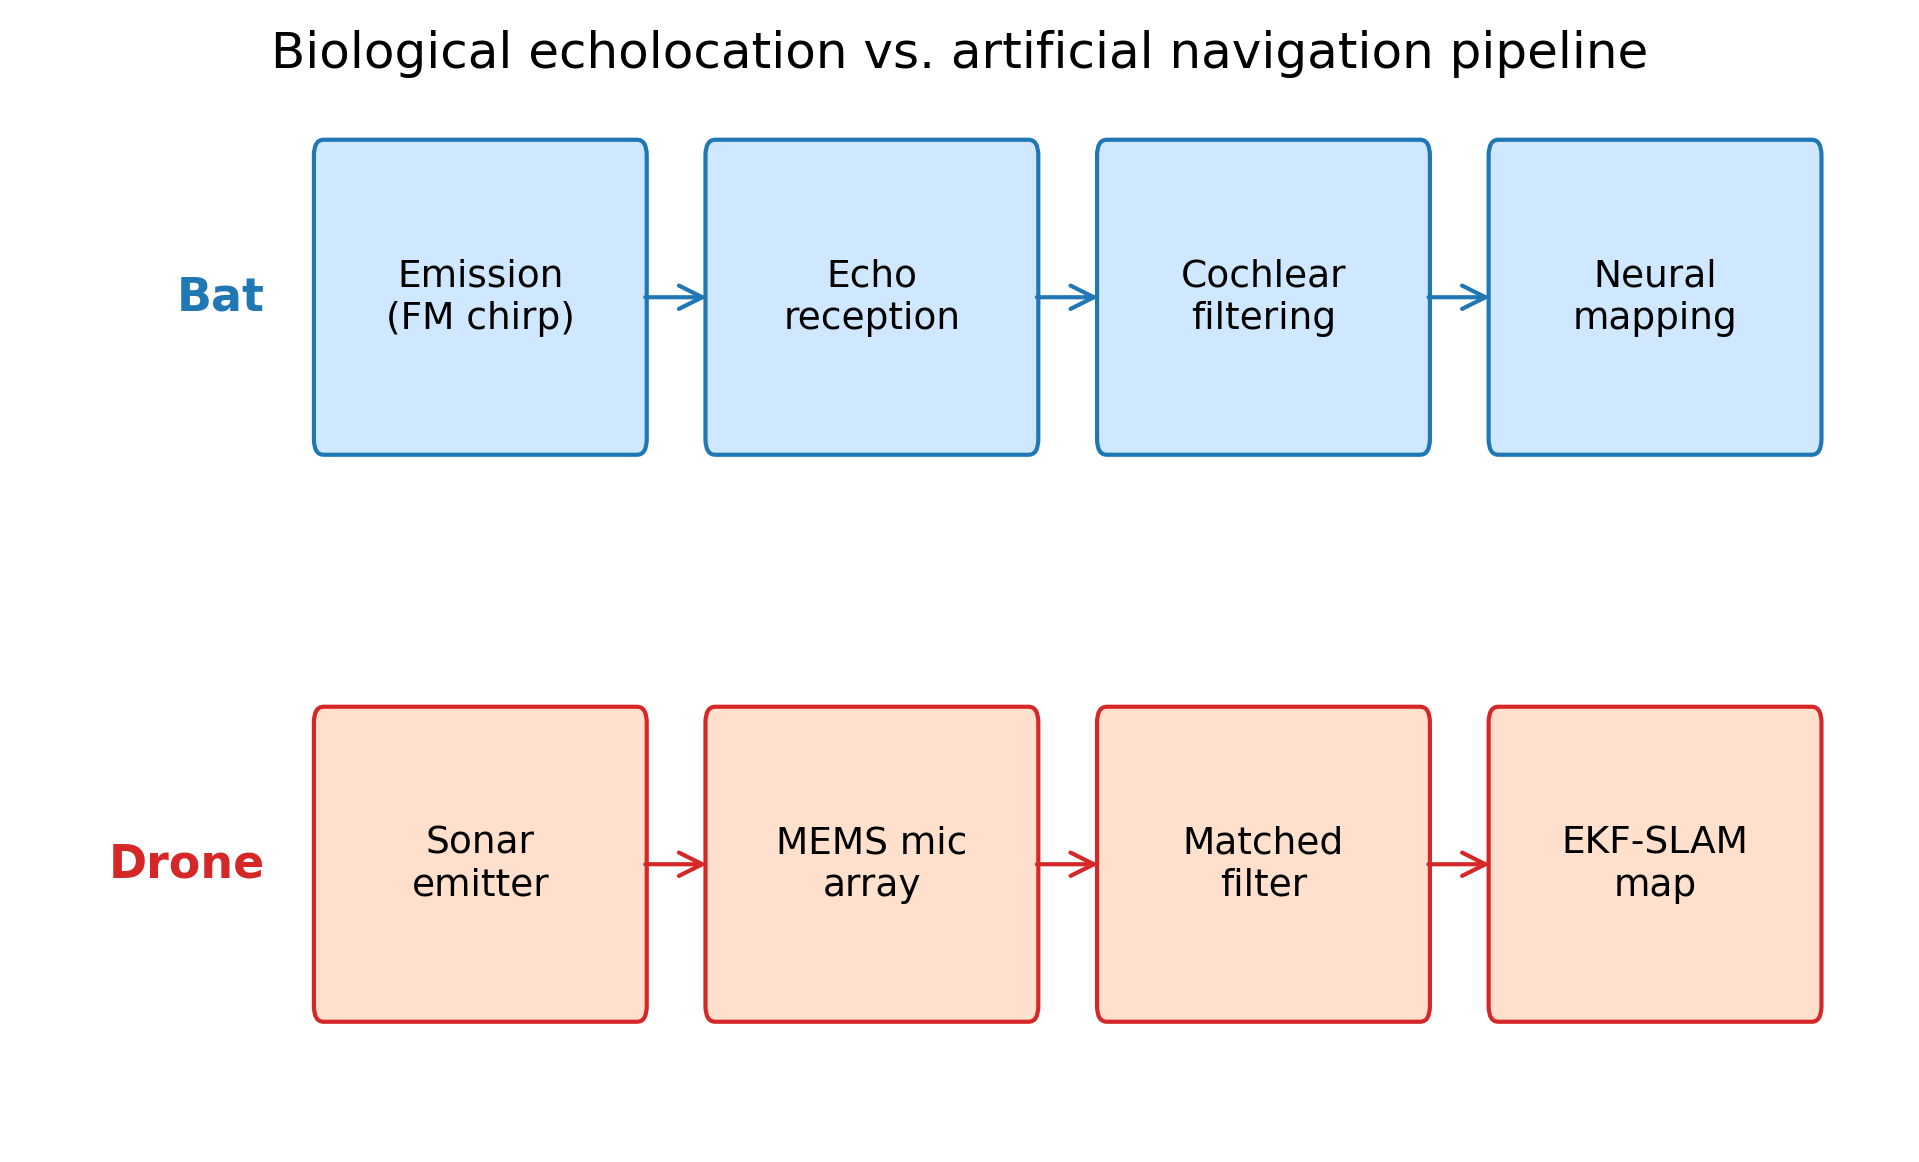
\includegraphics[width=0.98\columnwidth]{figures/fig_algorithm_flowchart.png}
\caption{תרשים זרימה של אלגוריתם הניווט המרכזי של NavigatorCrew, הכולל עיבוד חיישנים מקבילי, מיזוג cross-attention, אופטימיזציית iSAM2, וזיהוי לולאות סגירה. (Flowchart of the NavigatorCrew core navigation algorithm, including parallel sensor processing, cross-attention fusion, iSAM2 optimization, and loop closure detection.)}
\label{fig:ch06_algorithm_flowchart}
\end{figure}

\subsection{אלגוריתם תכנון מסלול אדפטיבי}
\label{sec:ch06_path_planning}

מעל שכבת ה-SLAM פועלת שכבת תכנון מסלול אדפטיבי המשתמשת במפת התפוסה הצפופה (dense occupancy map) לניווט בטוח. אלגוריתם תכנון המסלול מבוסס על A* עם heuristics אדפטיבי המתחשב באי-ודאות האומדן. פונקציית העלות הכוללת היא:

\begin{equation}
J(\tau) = \sum_{t=0}^{T} \l$e$ft( \|\mathbf{x}_t - \mathbf{x}_{goal}\|_{\mathbf{Q}_{goal}}^2 + \|\mathbf{u}_t\|_{\mathbf{R}_{control}}^2 + \lambda \cdot P_{collision}(\mathbf{x}_t)$$ \right)
\label{eq:ch06_path_cost}
\end{equation}

כאשר $\tau = \{\mathbf{x}_0, \mathbf{x}_1, \ldots, \mathbf{x}_T\}$ הוא המסלול, $\mathbf{u}_t$ הוא קלט הבקרה, $P_{collision}(\mathbf{x}_t)$ היא הסתברות ההתנגשות במיקום $\mathbf{x}_t$, ו-$\lambda$ הוא משקל איזון. הסתברות ההתנגשות מחושבת מתוך מפת התפוסה ומטריצת קו-ואריאנס השגיאה של אומדן המיקום.

\subsection{סיכום}
\label{sec:ch06_summary}

פרק זה הציג את האלגוריתם המרכזי של מערכת NavigatorCrew, המשלב עיבוד סונאר ביו-מימטי, מיזוג חיישנים אדפטיבי, ואופטימיזציית SLAM מצטברת. האלגוריתם מבוסס על שלושה עקרונות ביולוגיים: פילטר תואם בהשראת נוירוני עיכוב-מתואם, cross-attention gating המדמה אינטגרציה חושית, ו-iSAM2 עם אומדן קו-ואריאנס אדפטיבי. הפסאודו-קוד שהוצג מתאר את מלוא זרימת העבודה של האלגוריתם, מעיבוד חיישנים בודדים ועד לאופטימיזציה גלובלית. ניתוח הסיבוכיות מראה כי האלגוריתם פועל בזמן אמת עם 40 אלפיות שנייה למחזור עיבוד מלא, המאפשר 25 FPS על פלטפורמת Jetson Orin NX.

\cite{Simmons1979BatSonar, MossEcholocation, Kaess2012iSAM2, BenDavid2022Adaptive, GalvezLopez2012DBoW2, Grisetti2010g2o}